\documentclass[12pt]{article}
\usepackage{enumerate}
\usepackage{notes}
\usepackage{oxford}

\begin{document}

\section{A0 - Linear Algebra}
\begin{enumerate}
\item Why is $T$ an isomorphism here rather than merely a homomorphism? I guess the point is that
  $T$ need not be linear? But why need it be bijective? Also, what's the justification for the
  sentence ``Now $\bar T$ will be linear if it is well-defined.'' in the proof?
  \begin{mdframed}
    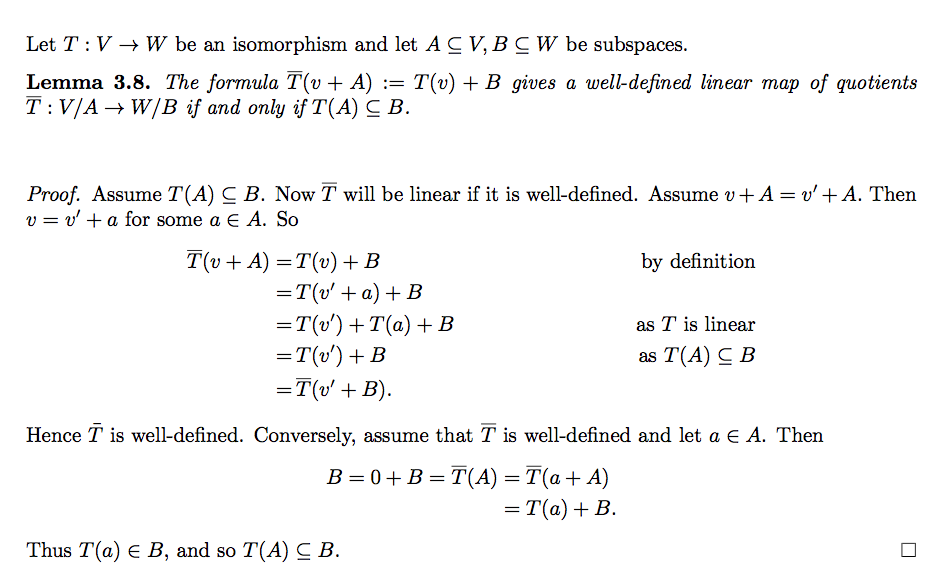
\includegraphics[width=400pt]{img/questions-linear-algebra-a0-induced-map-well-defined-theorem.png}
  \end{mdframed}
\item Why does the basis $\bar B$ of a quotient space not include the element $U$? (i.e. the coset
  which is the subspace/kernel). \blue{$\rightarrow$ because it's the additive identity}
  \begin{mdframed}
    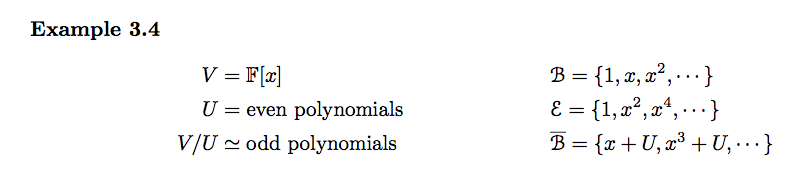
\includegraphics[width=400pt]{img/questions-linear-algebra-a0-basis-of-quotient-space.png}
  \end{mdframed}
  \blue{$\rightarrow$ because $U$ is the identity in the quotient space. Its coordinates are
    $(0, 0, ...)$ with respect to the basis $\bar B$. Let 0 be the additive identity in the field
    $\F$. Then $0v = \vec 0$ for all $v$, where $\vec 0$ is the additive identity in the abelian
    group of the vector space.}
\item Can a normal subgroup be the kernel of more than one homomorphism? I think so. If so, are the
  images of those homomorphisms isomorphic? Presumably. $\rightarrow$ \blue{yep}
\item Are the elements of a vector space always ``array-like'', allowing ``componentwise''
  operations? (i.e. functions are array like because they can be considered to be an indexed set of
  tuples.) \blue{$\rightarrow$ Does every vector space have a basis \blue{$\rightarrow$ Axiom of Choice,
    Zorn's Lemma.}}
\item When is multiplication of functions defined to be composition versus componentwise
  multiplication? $(fg)(x) := f(g(x))$ vs $(fg)(x) := f(x)g(x)$. \blue{$\rightarrow$ Either might
    make sense.}
\item In $\R^3$ a set of basis vectors have no natural order. But in e.g. the space of functions on
  $(0, 1)$ the basis vectors would have a natural order I think. What distinction is being
  identified there? \blue{$\rightarrow$ well, $R^n$ basis vectors do have an order. But yes there
    are bases of vector spaces with no natural order (e.g. space of functions on a set with no
    ordering).}
\item Conrad says
  \begin{quote}
    ``there is a nonzero monic polynomial that kills a linear operator A''.
  \end{quote}
  Now in general applying a polynomial to a linear transformation (``operator'') is not
  well-defined (choice of basis $\rightarrow$ different matrix $\rightarrow$ different
  result). However, (theorem) if the polynomial kills a matrix $A$ then it will also kill $A$ after
  any change-of-basis. Because $(P^\1AP)^k = (P^\1AP)(P^\1AP)\cdots (P^\1AP) = (P^\1A^kP)$
  ...hmm. Not sure I understand this:
  \begin{mdframed}
    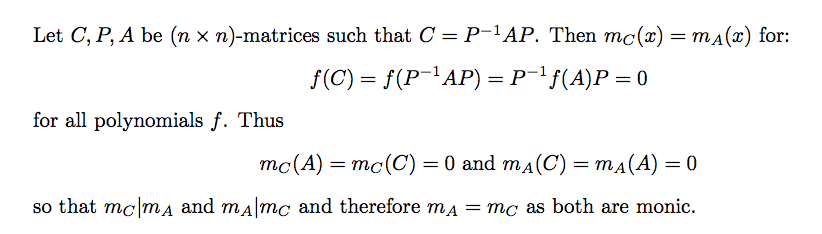
\includegraphics[width=400pt]{img/questions-linear-algebra-a0-minimal-polynomial.png}
  \end{mdframed}
  \blue{$\rightarrow$ Ultimately feeding a transformation to a polynomial outputs another
    transformation; it's basis-independent. Algebraically,
    $f(P^\1AP) = \sum_i a_i(P^\1AP)^i = \sum_i a_iP^\1A^iP = P^\1\Big(\sum_ia_iA^i\Big)P =
    P^\1f(A)P$.}
\item What is an example of a subring that is not an ideal?\\
  \url{https://math.stackexchange.com/questions/1098217/subring-which-is-not-an-ideal}
\item Definition of direct sum\\
  Halmos says
  \begin{mdframed}
    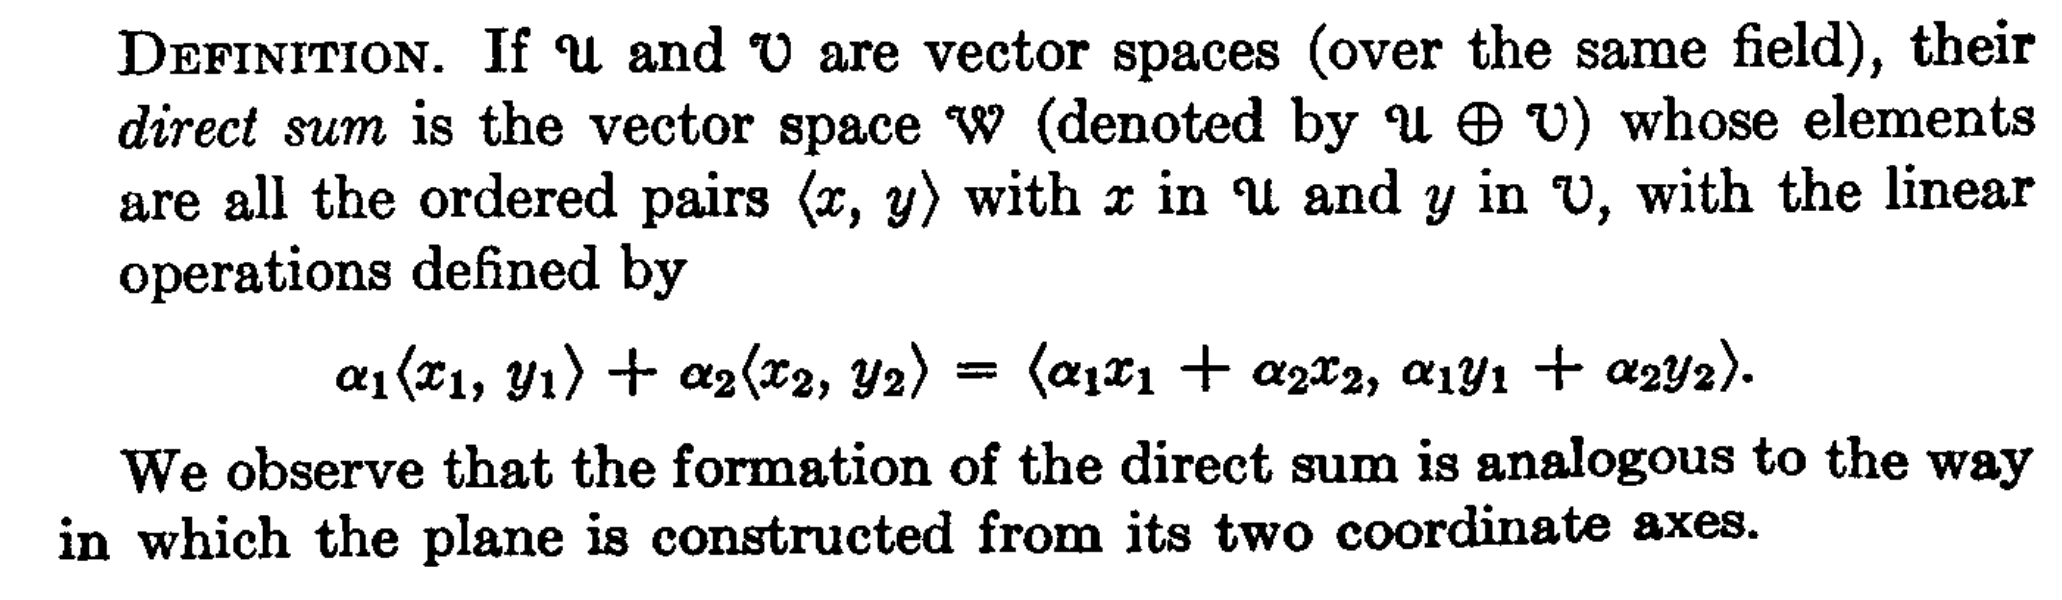
\includegraphics[width=400pt]{img/questions-linear-algebra-a0-direct-sum-halmos.png}
  \end{mdframed}
  Lauder says
  \begin{mdframed}
    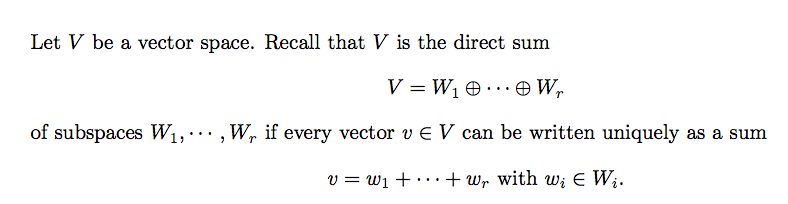
\includegraphics[width=400pt]{img/questions-linear-algebra-a0-direct-sum-lauder.png}
  \end{mdframed}
\item ``Linear operator'' vs ``Linear transformation''\\
  Conrad uses ``linear operator'' whereas Oxford notes use ``linear transformation'' for what is
  AFAIK the same concept?
  \begin{mdframed}
    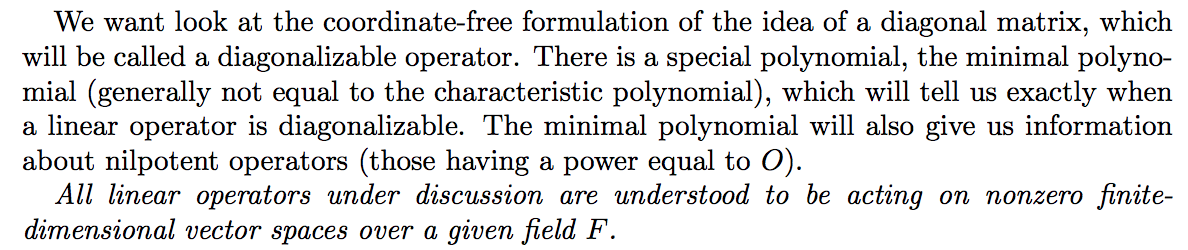
\includegraphics[width=400pt]{img/questions-linear-algebra-a0-operator-halmos.png}
  \end{mdframed}
\end{enumerate}


\section{A1 - Differential Equations}

\begin{enumerate}
\item 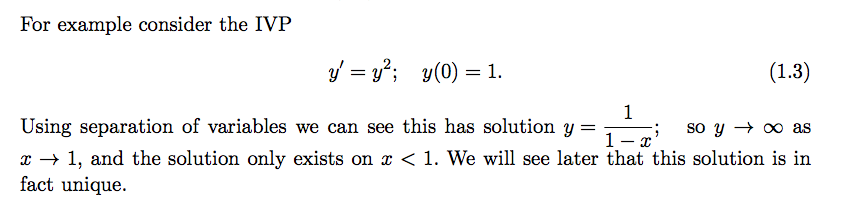
\includegraphics[width=400pt]{img/questions-differential-equations-a1-warning.png}\\
  Why does solution not exist for $x > 1$?
\end{enumerate}

\section*{A2 - Metric Spaces}


\begin{enumerate}
\item What do you think about when you think about the Cauchy-Schwarz inequality? (E.g. something
  geometric or algebraic?)
\item Other than the positive reals, what sets can be the codomain of a metric?
\item Are open sets always spherical in a metric space?
  \begin{mdframed}
    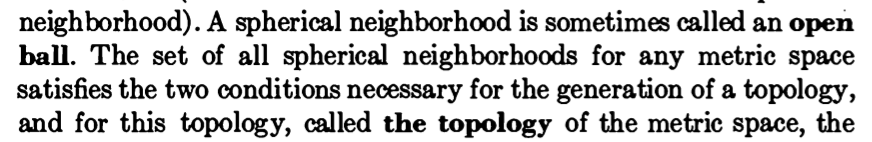
\includegraphics[width=400pt]{img/questions-metric-space-open-sets-gelbaum.png}
  \end{mdframed}
\newpage
\item I think that $B(x, r) \subseteq B(a, \epsilon)$ is sufficient but not necessary, in that if a
  ball of radius $r$ doesn't fit, then we could always seek a ball of smaller radius. Right?
  \begin{mdframed}
    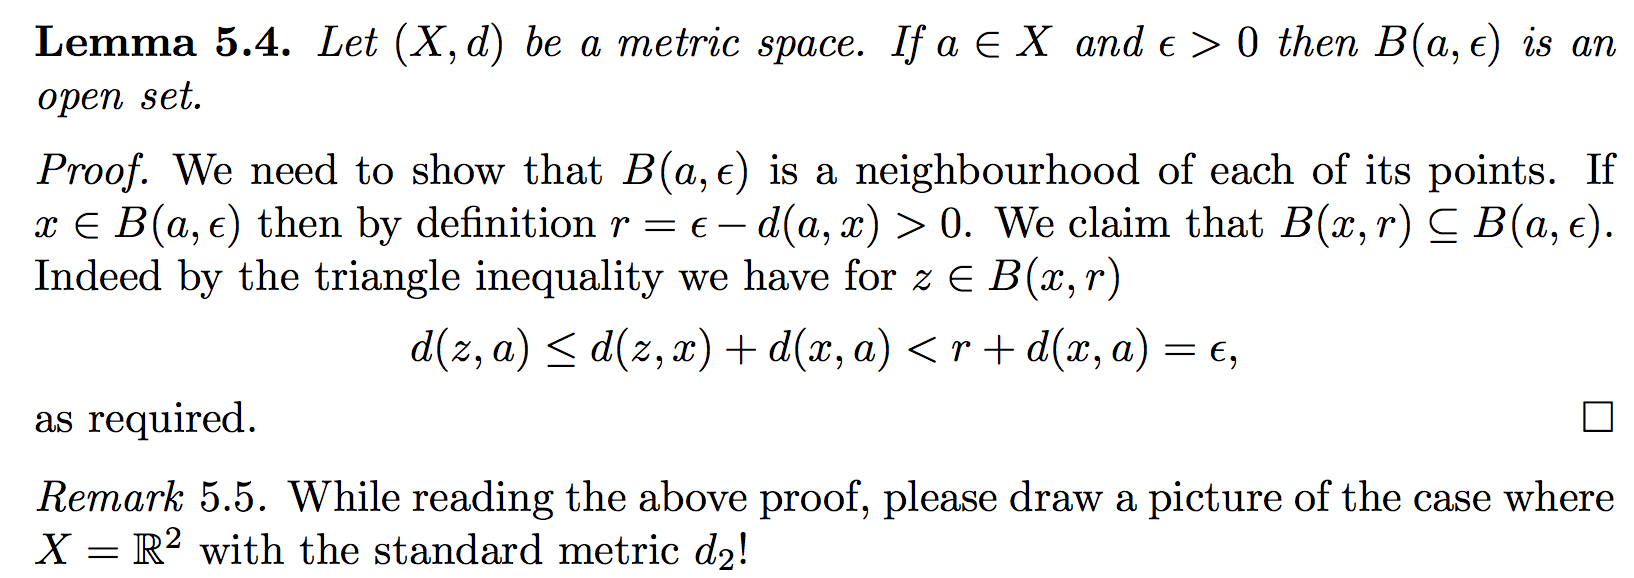
\includegraphics[width=400pt]{img/questions-oxford-a2-ball-is-open-proof.png}\\
    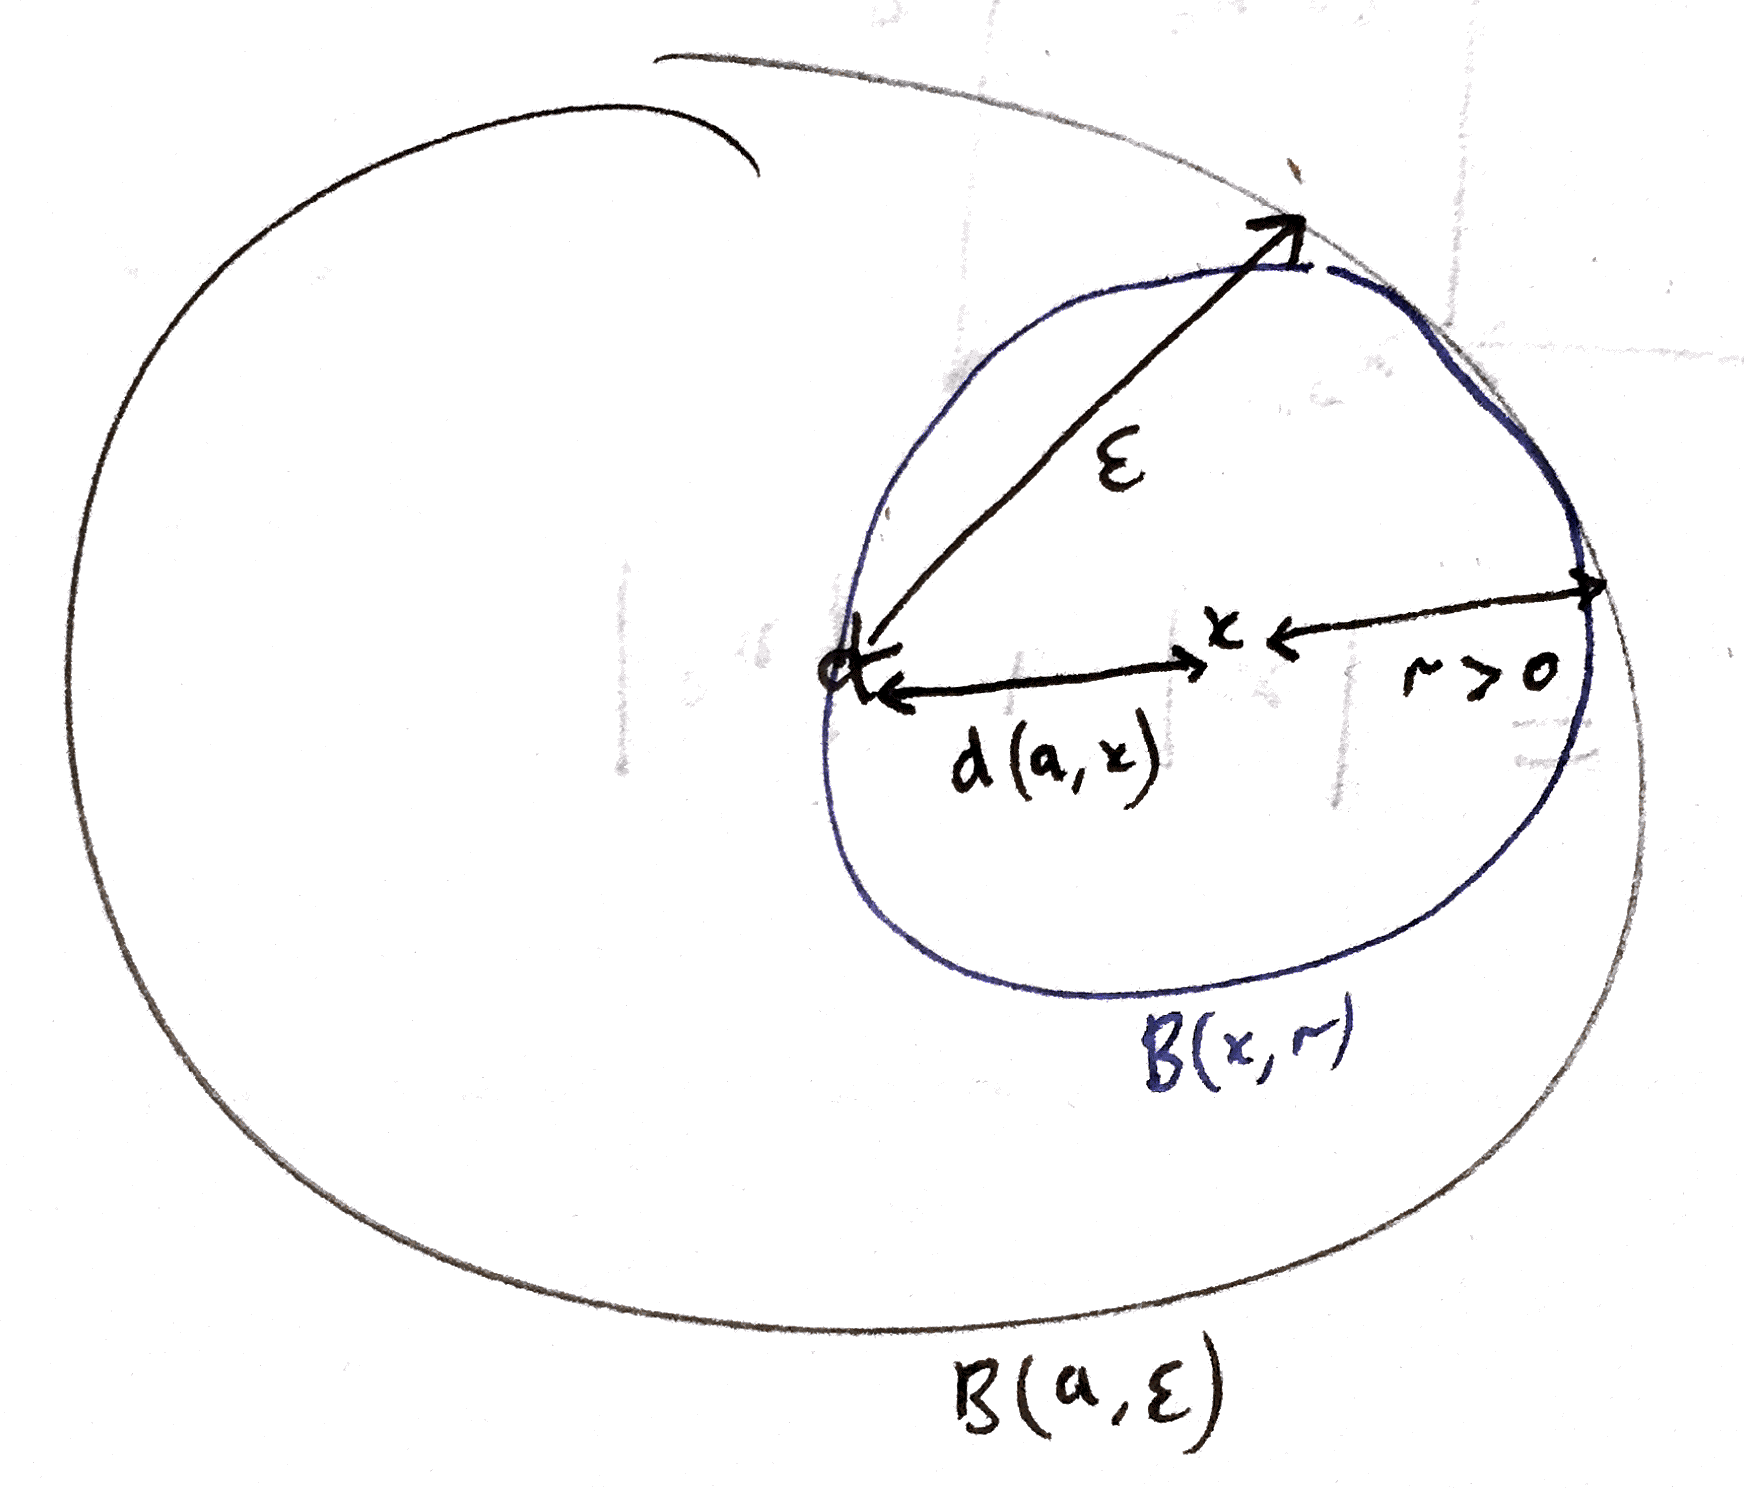
\includegraphics[width=200pt]{img/questions-oxford-a2-ball-is-open-proof-diagram.png}
  \end{mdframed}
\item Understand the forward part of this proof. (I understand the converse.)
  \begin{mdframed}
    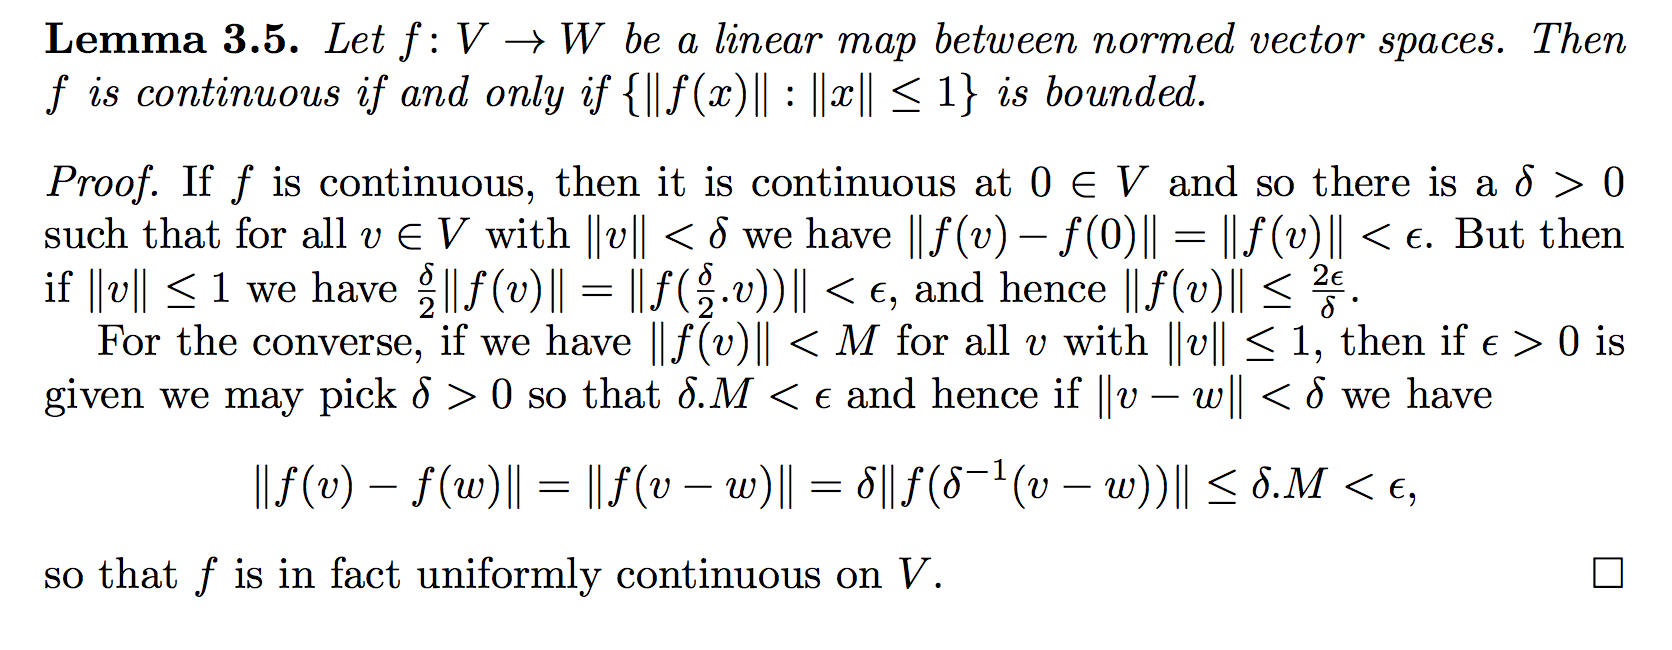
\includegraphics[width=400pt]{img/questions-oxford-a2-linear-transformation-continuity.png}
  \end{mdframed}
\end{enumerate}

\section*{Misc}
\begin{enumerate}
\item When giving a definition should one say
  \begin{quote}
    $f$ is a (thing being defined) if (some condition).
  \end{quote}
  Or should that be if and only if?
\end{enumerate}

\end{document}
